\let\negmedspace\undefined
\let\negthickspace\undefined
\documentclass[journal]{IEEEtran}
\usepackage[a5paper, margin=10mm, onecolumn]{geometry}
%\usepackage{lmodern} % Ensure lmodern is loaded for pdflatex
\usepackage{tfrupee} % Include tfrupee package

\setlength{\headheight}{1cm} % Set the height of the header box
\setlength{\headsep}{0mm}  % Set the distance between the header box and the top of the text

\usepackage{gvv-book}
\usepackage{gvv}
\usepackage{cite}
\usepackage{amsmath,amssymb,amsfonts,amsthm}
\usepackage{algorithmic}
\usepackage{graphicx}
\usepackage{textcomp}
\usepackage{xcolor}
\usepackage{txfonts}
\usepackage{listings}
\usepackage{enumitem}
\usepackage{mathtools}
\usepackage{gensymb}
\usepackage{comment}
\usepackage[breaklinks=true]{hyperref}
\usepackage{tkz-euclide} 
\usepackage{listings}
% \usepackage{gvv}                                        
\def\inputGnumericTable{}                                 
\usepackage[latin1]{inputenc}                                
\usepackage{color}                                            
\usepackage{array}                                            
\usepackage{longtable}                                       
\usepackage{calc}                                             
\usepackage{multirow}                                         
\usepackage{hhline}                                           
\usepackage{ifthen}                                           
\usepackage{lscape}

% Marks the beginning of the document
\begin{document} 
\bibliographystyle{IEEEtran}
\vspace{3cm}

\title{4-4.2-5}
\author{EE24BTECH11029- JANAGANI SHRETHAN REDDY}
\maketitle
\bigskip
\renewcommand{\thefigure}{\theenumi}
\renewcommand{\thetable}{\theenumi}
\textbf{Question:}
Find the direction and normal vectors of the line $2x=-5y$.\\
\solution\\
%\begin{table}[h!]
 %\centering
 %\begin{tabular}{|c|c|c|}
\hline
variable& Description&formula
\\\hline
\multirow{3}{1em}\\A$\brak{2,3}$&one end of the line segment&$-$
\\\hline
B$\brak{7,8}$&another end of the line segment&$-$
\\\hline
P $\brak{4,5}$&divides$\vec{A}$and $\vec{B}$ in the ratio $k\colon1$&$ P=\frac{\vec{A}+k\vec{B}}{k+1}$
\\\hline
\end{tabular}

 %\caption{variable used}
%\end{table}\\
\begin{align}
    y&=sx+c\\
   \implies\myvec{x\\y}&=\myvec{x\\sx+c}\\
    \implies\myvec{x\\y}&=\myvec{0\\c}+x\myvec{1\\s}\\
    m&=\myvec{1\\s}\\
    m^Tn&=0\\
    n&=\myvec{-s\\1}
\end{align}
where m,n are direction and normal vectors.
\begin{align}
    -5y&=2x\\
    y&=\frac{2}{-5}x\\
    \myvec{x\\y}&=\myvec{x\\ \frac{2}{-5}x}\\
    \myvec{x\\y}&=x\myvec{1\\ \frac{2}{-5}}\\
    m&=\myvec{1\\s}\\
    \implies m&=\myvec{1\\ -\frac{2}{5}}\\
    m^Tn&=0\\
    n&=\myvec{-s\\1}\\
  \implies  n&=\myvec{\frac{2}{5}\\1}
\end{align}
 \begin{figure}[h!]
  \centering
  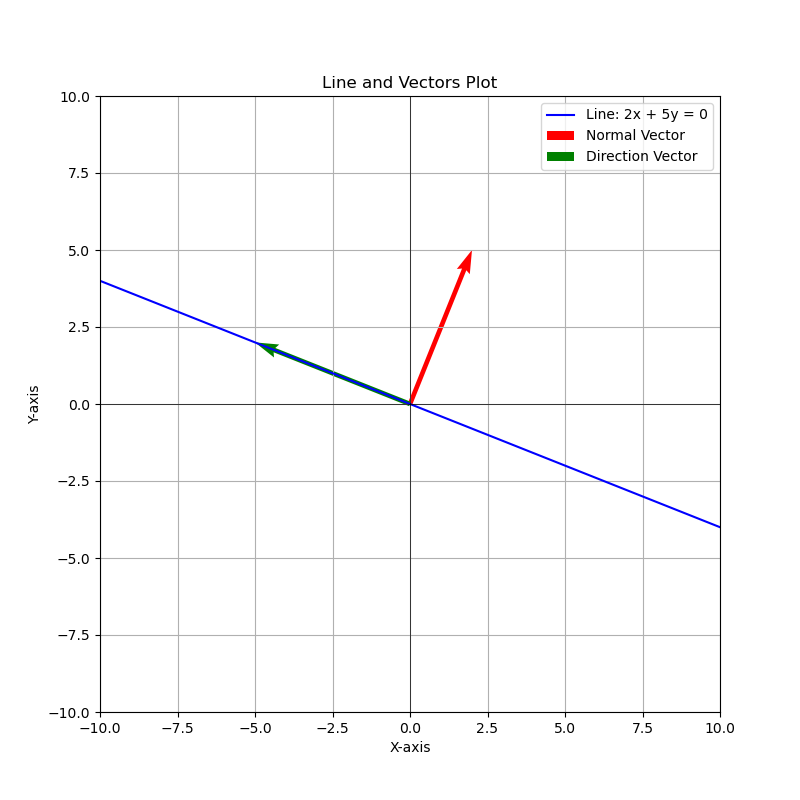
\includegraphics[width=1\linewidth]{fig/fig.png}
  \caption{plot of direction and normal vector}
 \end{figure}
\end{document}
